\begin{figure}
    \centering
    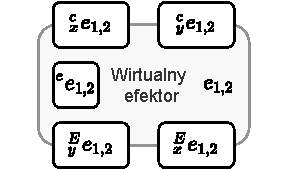
\includegraphics[width=0.75\columnwidth]{figures/ISR-ve-gripper-model.pdf}
    \label{fig:model-vr-camera}
    \caption{Struktura ogólna wirtualnego efektora chwytaka dwustanowego}
\end{figure}

\begin{figure}
    \centering
    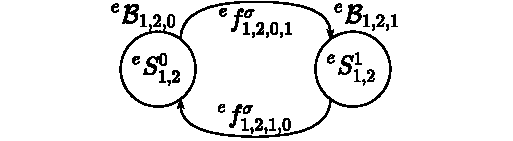
\includegraphics[width=\columnwidth]{figures/ISR-ve-gripper-behaviours.pdf}
    \label{fig:zachowania-ve-gripper}
    \caption{Automat zachowań wirtualnego efektora chwytaka dwustanowego}
\end{figure}

Efektor wirtualny chwytaka (slajdy 113-119):
\begin{itemize}
    \item bufor wejściowy od podsystemu sterowania: stan pożądany,
    \item bufor wyjściowy do podsystemu sterowania: stan aktualny,
    \item bufor wejściowy od rzeczywistego efektora: stan aktualny,
    \item bufor wyjściowy do rzeczywistego efektora: stan pożądany.
\end{itemize}


Zachowania:
\begin{itemize}
    \item ${}^{e}\mathcal{B}_{1,2,0}$ - idle,
    \item ${}^{e}\mathcal{B}_{1,2,1}$ - move.
\end{itemize}